%%%%%%%%%%%%%%%%%%%%%%%%%%%%%%%%%%%%%%%%%%%
%
% Consultar o ficheiro README
%
%%%%%%%%%%%%%%%%%%%%%%%%%%%%%%%%%%%%%%%%%%%

\documentclass[pdflatex,compress]{beamer}


\usetheme[dark,framenumber,totalframenumber]{UBI}


% Fonts, the official UBI font. O tipo de letra é o Georgia da Microsoft Office. O tipo de letra é o definido no GUIA DE NORMAS DE IDENTIDADE da UBI
\usepackage{fontspec,microtype}
\usepackage{unicode-math}
\usepackage{pifont}
\defaultfontfeatures{Ligatures={TeX},Renderer=Basic}
\setmainfont[Ligatures={TeX,Historic}]{Georgia}
\setsansfont{Georgia} 
\setmonofont{Georgia}
%%%%%%%%%%%%%%%%%%


%\usepackage{lipsum}

\title{Preventing Data Exfiltration inside Virtual Machines}
\subtitle{eBPF-based approach}

\author{Supervisor: André Passos\\
Orientador: Prof. Doutora Manuela Pereira\\
Co-Orientador: Prof. Doutor Simão Melo de Sousa\\
\bigskip\bigskip 
Orientando: Carlos Pinto}

\begin{document}

% ----------------------------------------------------------------------------
% *** Titlepage <<<
% ----------------------------------------------------------------------------
\maketitle
% ----------------------------------------------------------------------------
% *** END of Titlepage >>>
% ----------------------------------------------------------------------------

\section{My section}
\subsection{My subsection}

% ----------------------------------------------------------------------------
% *** Test frame <<<
% ----------------------------------------------------------------------------
\begin{frame}
\frametitle{Problema}

O problema abordado nesta tese é o da prevenção de data exfiltration. 
\pause \bigskip

Data exfiltration pode ser caracterizado como: 
\begin{enumerate}
    \pause
    \item Transferência não autorizada de dados de um computador ou outro dispostivo. 
        \pause 
    \item Envolve a cópia ilícita de dados, com agência maliciosa. 
        \pause
    \item Pode ser conduzido de forma manual ou de forma automatizada usando malware. 
\end{enumerate}

\end{frame}

\begin{frame}
\frametitle{Problema II}

A possibilidade de dados poderem ser transferidos sem autorização é particularmente gravosa para empresas, visto poderem incorrer não só em danos monetários, e de roubo de propriedade intelectual, mas também poderem ver a sua credibilidade afetada caso tal aconteça. 

\end{frame}


\begin{frame}

\frametitle{Solução Proposta}

Desenvolver uma aplicação que faça uso de kernel-based security, com base em eBPF, de modo a prevenir data exfiltration em máquinas virtuais.

\end{frame}

\subsection{Conceitos e Estado da Arte}


\begin{frame}
\frametitle{Conceitos Base}

\pause
\begin{exampleblock}{Linux Kernel}
    O Kernel de Linux é o componente base do sistema operativo Linux, servindo como mediador entre software e hardware.
\end{exampleblock}

\bigskip

\pause
\begin{exampleblock}{eBPF}
    eBPF é uma tecnologia que permite correr programas dentro do kernel sem modificar o mesmo.
\end{exampleblock}

\end{frame}
% ----------------------------------------------------------------------------

\begin{frame}
\frametitle{Linux Kernel}

\begin{exampleblock}{Tarefas do Kernel}
    \begin{itemize}
        \pause
        \item Gestão de processos. 
        \pause    
    \item Gestão de memória. 
        \pause
    \item Drivers de dispositivos. 
        \pause
        \item\textbf{System Calls e Segurança.}
    \end{itemize}
\end{exampleblock}


\end{frame}
% ----------------------------------------------------------------------------
% *** END of Test frame with Math >>>
% ----------------------------------------------------------------------------

\begin{frame}
\frametitle{Kernel Space}
\bigskip
\begin{figure}[t]
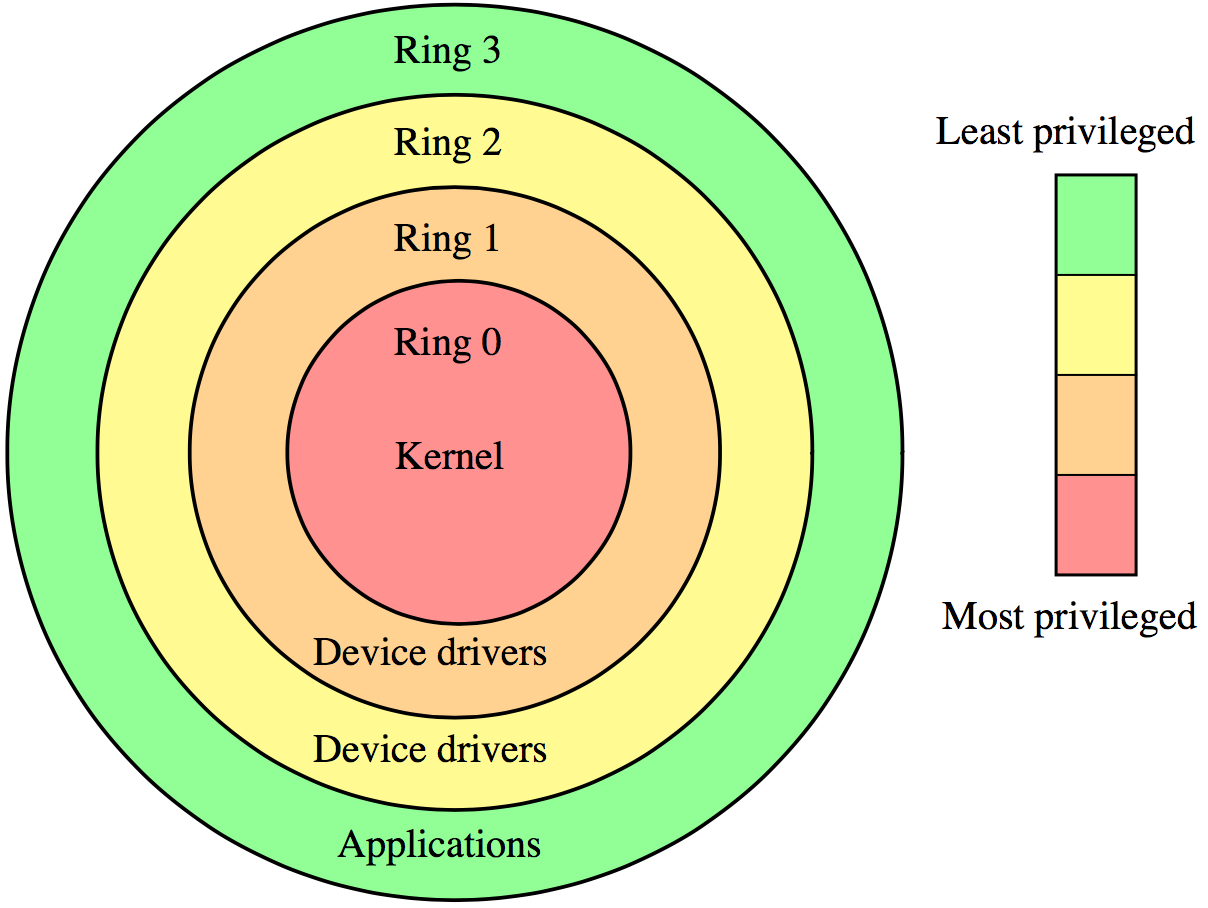
\includegraphics[scale=0.15]{images/kernel.png}
\centering
\end{figure}
\end{frame}

\begin{frame}
\frametitle{System Calls}
\bigskip
\begin{figure}[t]
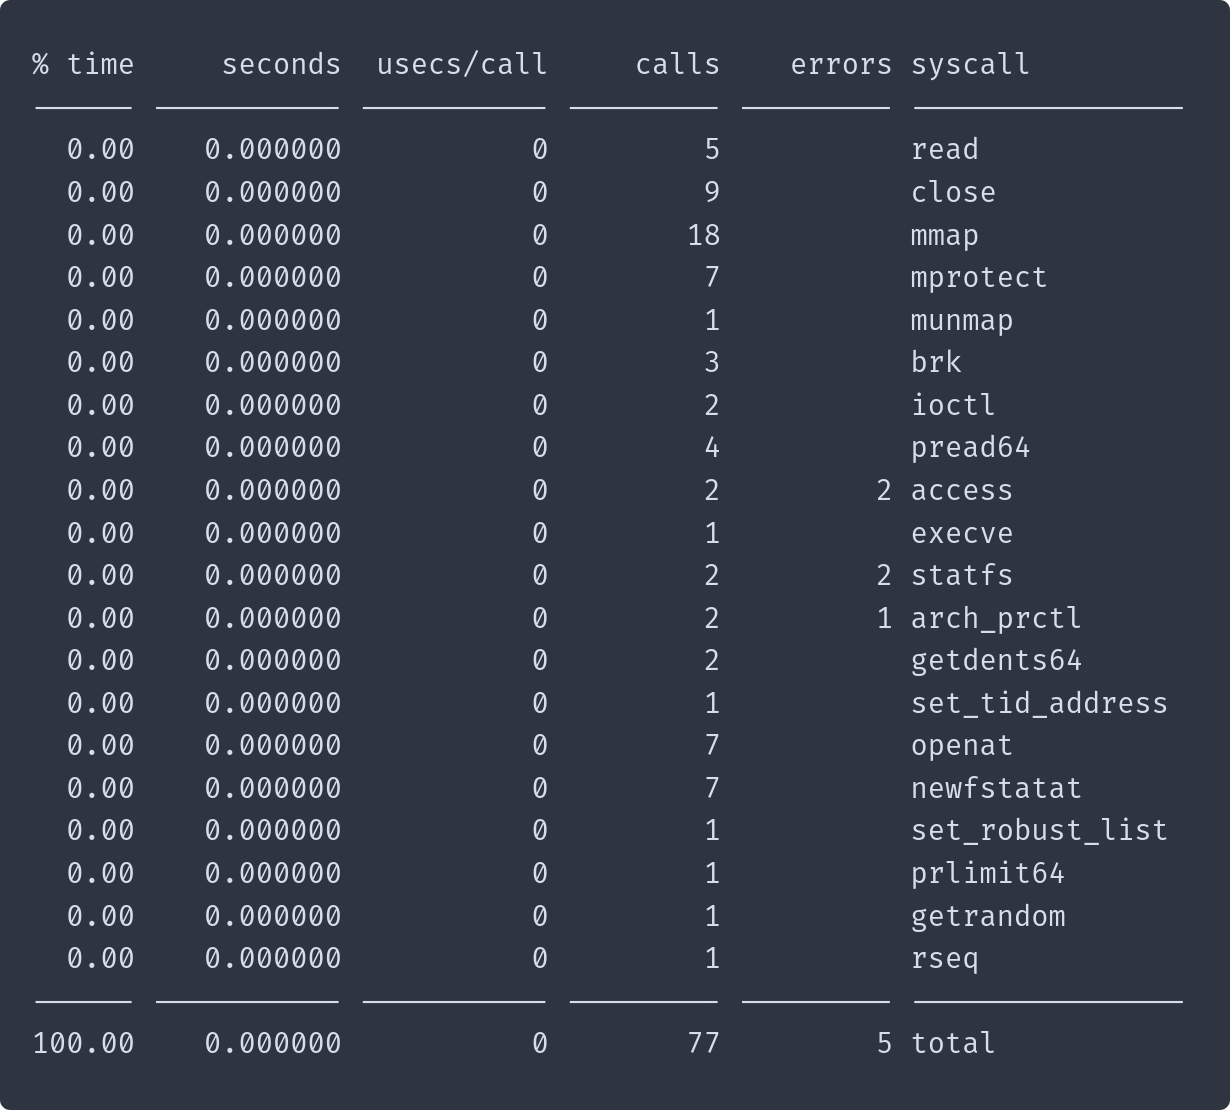
\includegraphics[width=8cm, height=6cm]{images/strace2.png}
\centering
\end{figure}
\end{frame}

\begin{frame}
\frametitle{eBPF}

\begin{figure}[x]
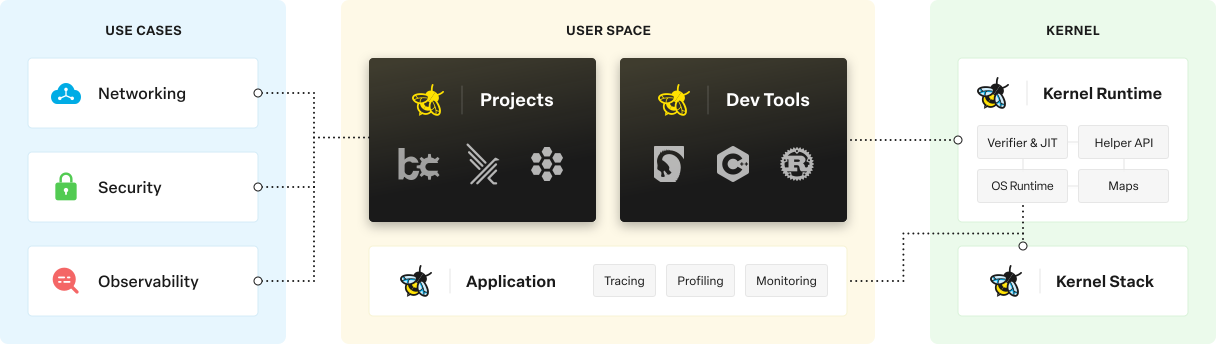
\includegraphics[scale=0.25]{images/bpf.png}
\centering
\end{figure}
\end{frame}
% ----------------------------------------------------------------------------
% *** Test frame with Environments <<<
% ----------------------------------------------------------------------------

\begin{frame}
\frametitle{Kernel VS User Space}


\begin{figure}[x]
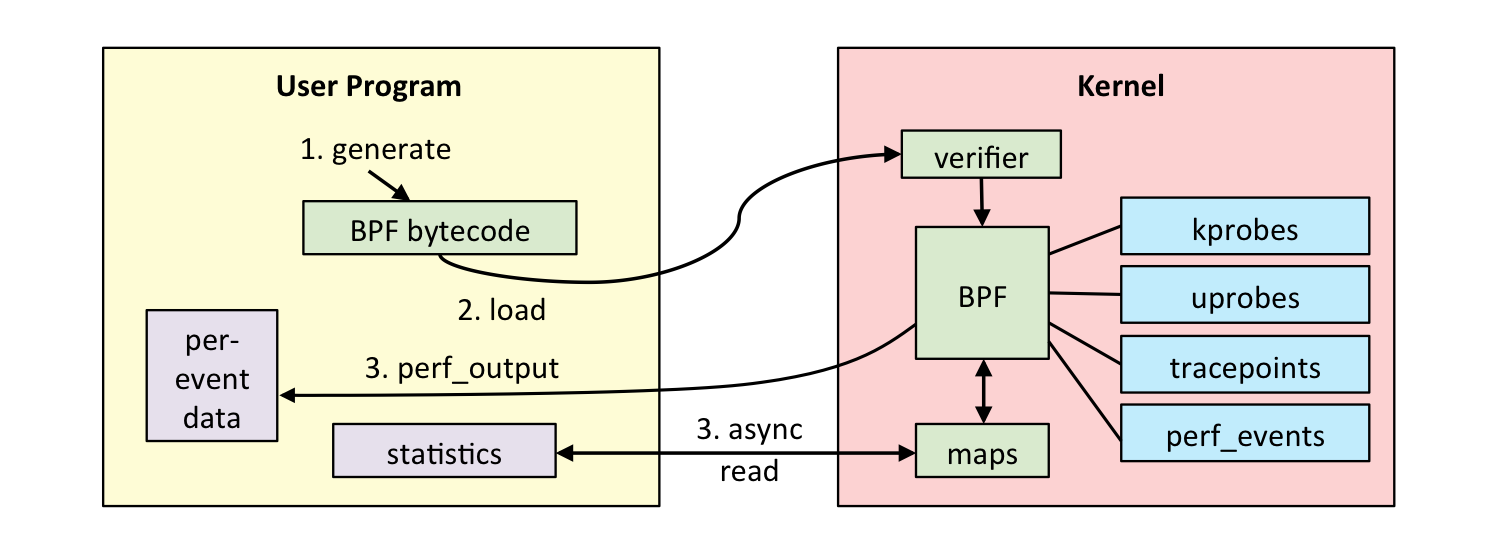
\includegraphics[scale=0.21]{images/internal.png}
\centering
\end{figure}

\end{frame}

% \begin{frame}
% \frametitle{Overview}
%
%
% \begin{figure}[x]
% 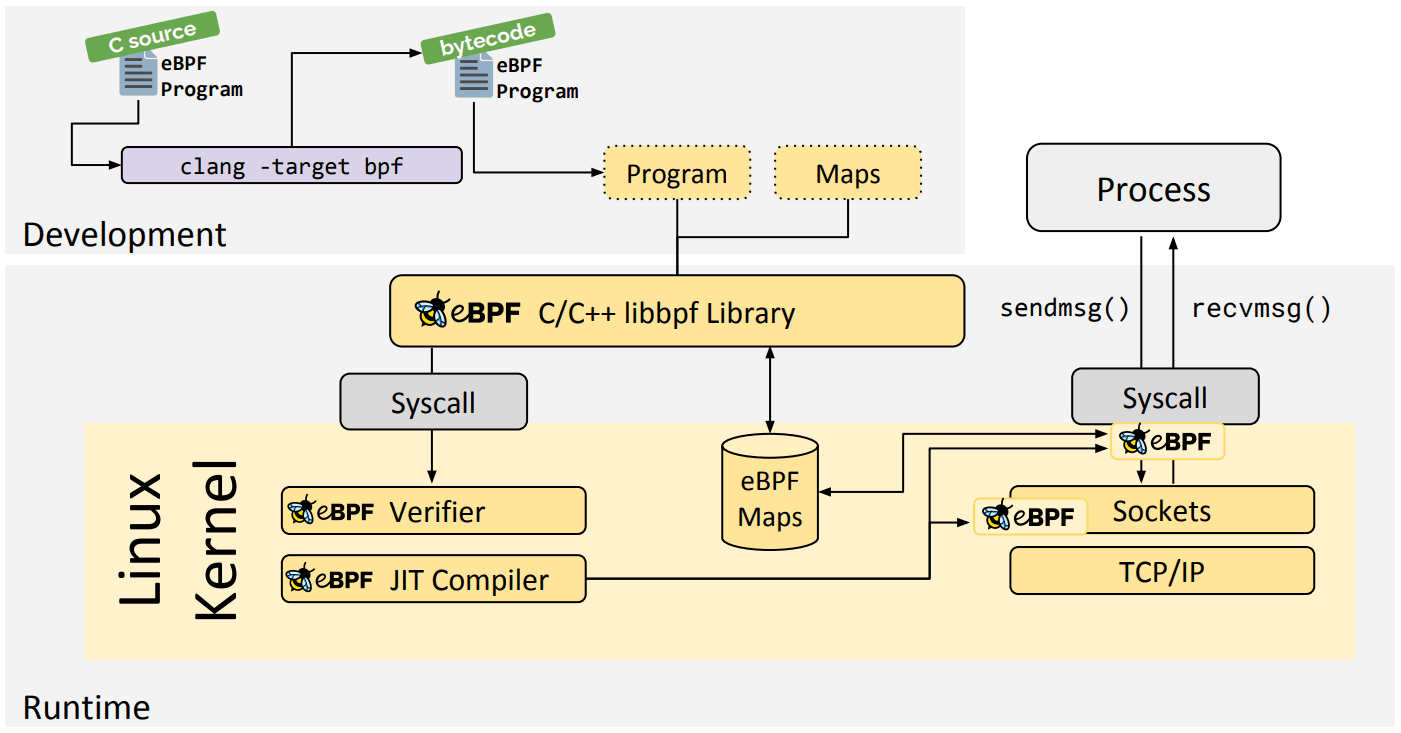
\includegraphics[scale=0.21]{libbpf.png}
% \centering
% \end{figure}
%
% \end{frame}


\begin{frame}
\frametitle{Verificação}


\begin{figure}[x]
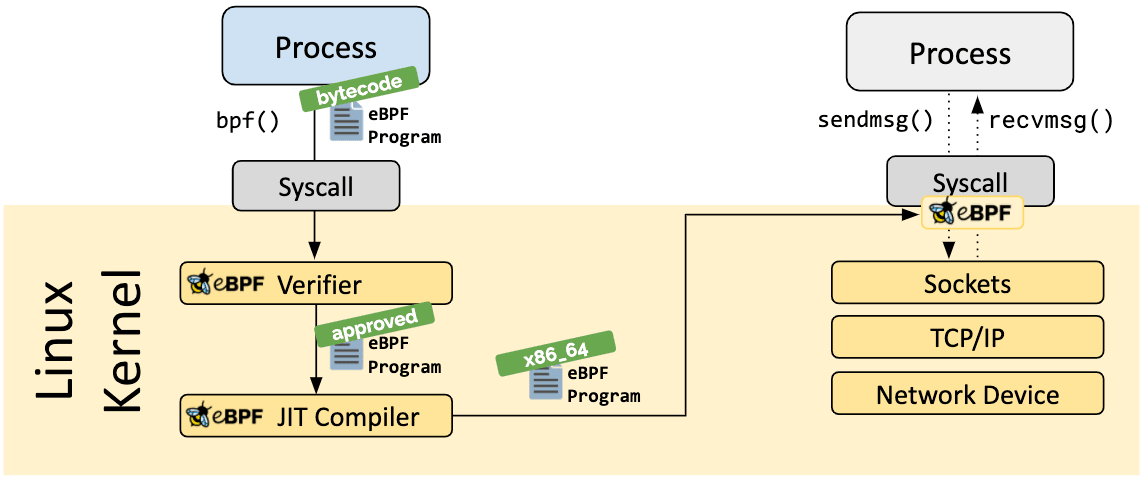
\includegraphics[scale=0.25]{images/verifier.png}
\centering
\end{figure}

\end{frame}


\begin{frame}
\frametitle{Mapas eBPF}


\begin{figure}[x]
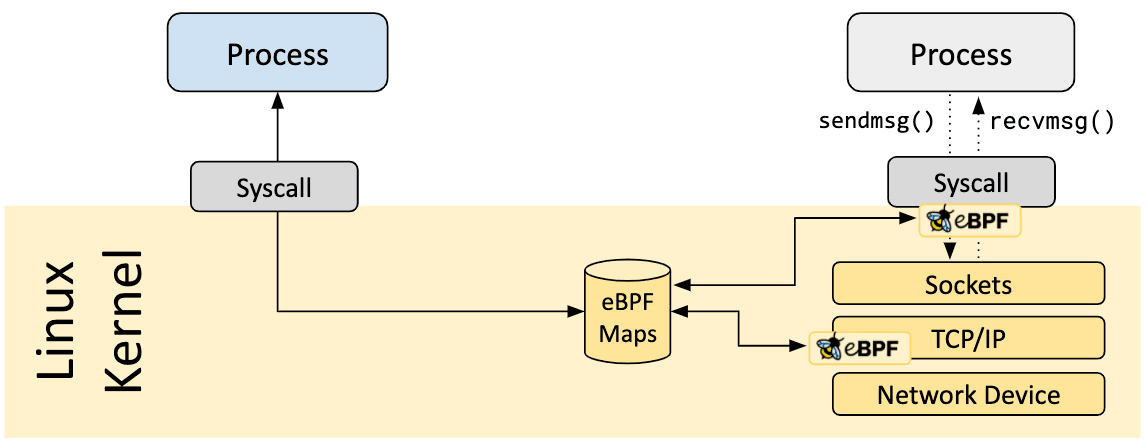
\includegraphics[scale=0.25]{images/map.png}
\centering
\end{figure}

\end{frame}


\begin{frame}
\frametitle{Estado da Arte}

\begin{exampleblock}{Ferramentas}
    \begin{itemize}
        \pause
        \item Seccomp-bpf
        \pause
        \item Tetragon
    \end{itemize}
\end{exampleblock}

\end{frame}


\begin{frame}
\frametitle{Seccomp-bpf}

A ferramenta \emph{seccomp-bpf} é uma extensão ao \emph{seccomp} que permite filtrar as \emph{syscalls} a partir de um programa BPF.

É mais flexível que o \emph{seccomp} original, que permitia apenas quatro \emph{syscalls}.  


\end{frame}


\begin{frame}
\frametitle{Tetragon}

%Falar das 3, tetragon, bpf lsm e seccomp-bpf

\begin{figure}[x]
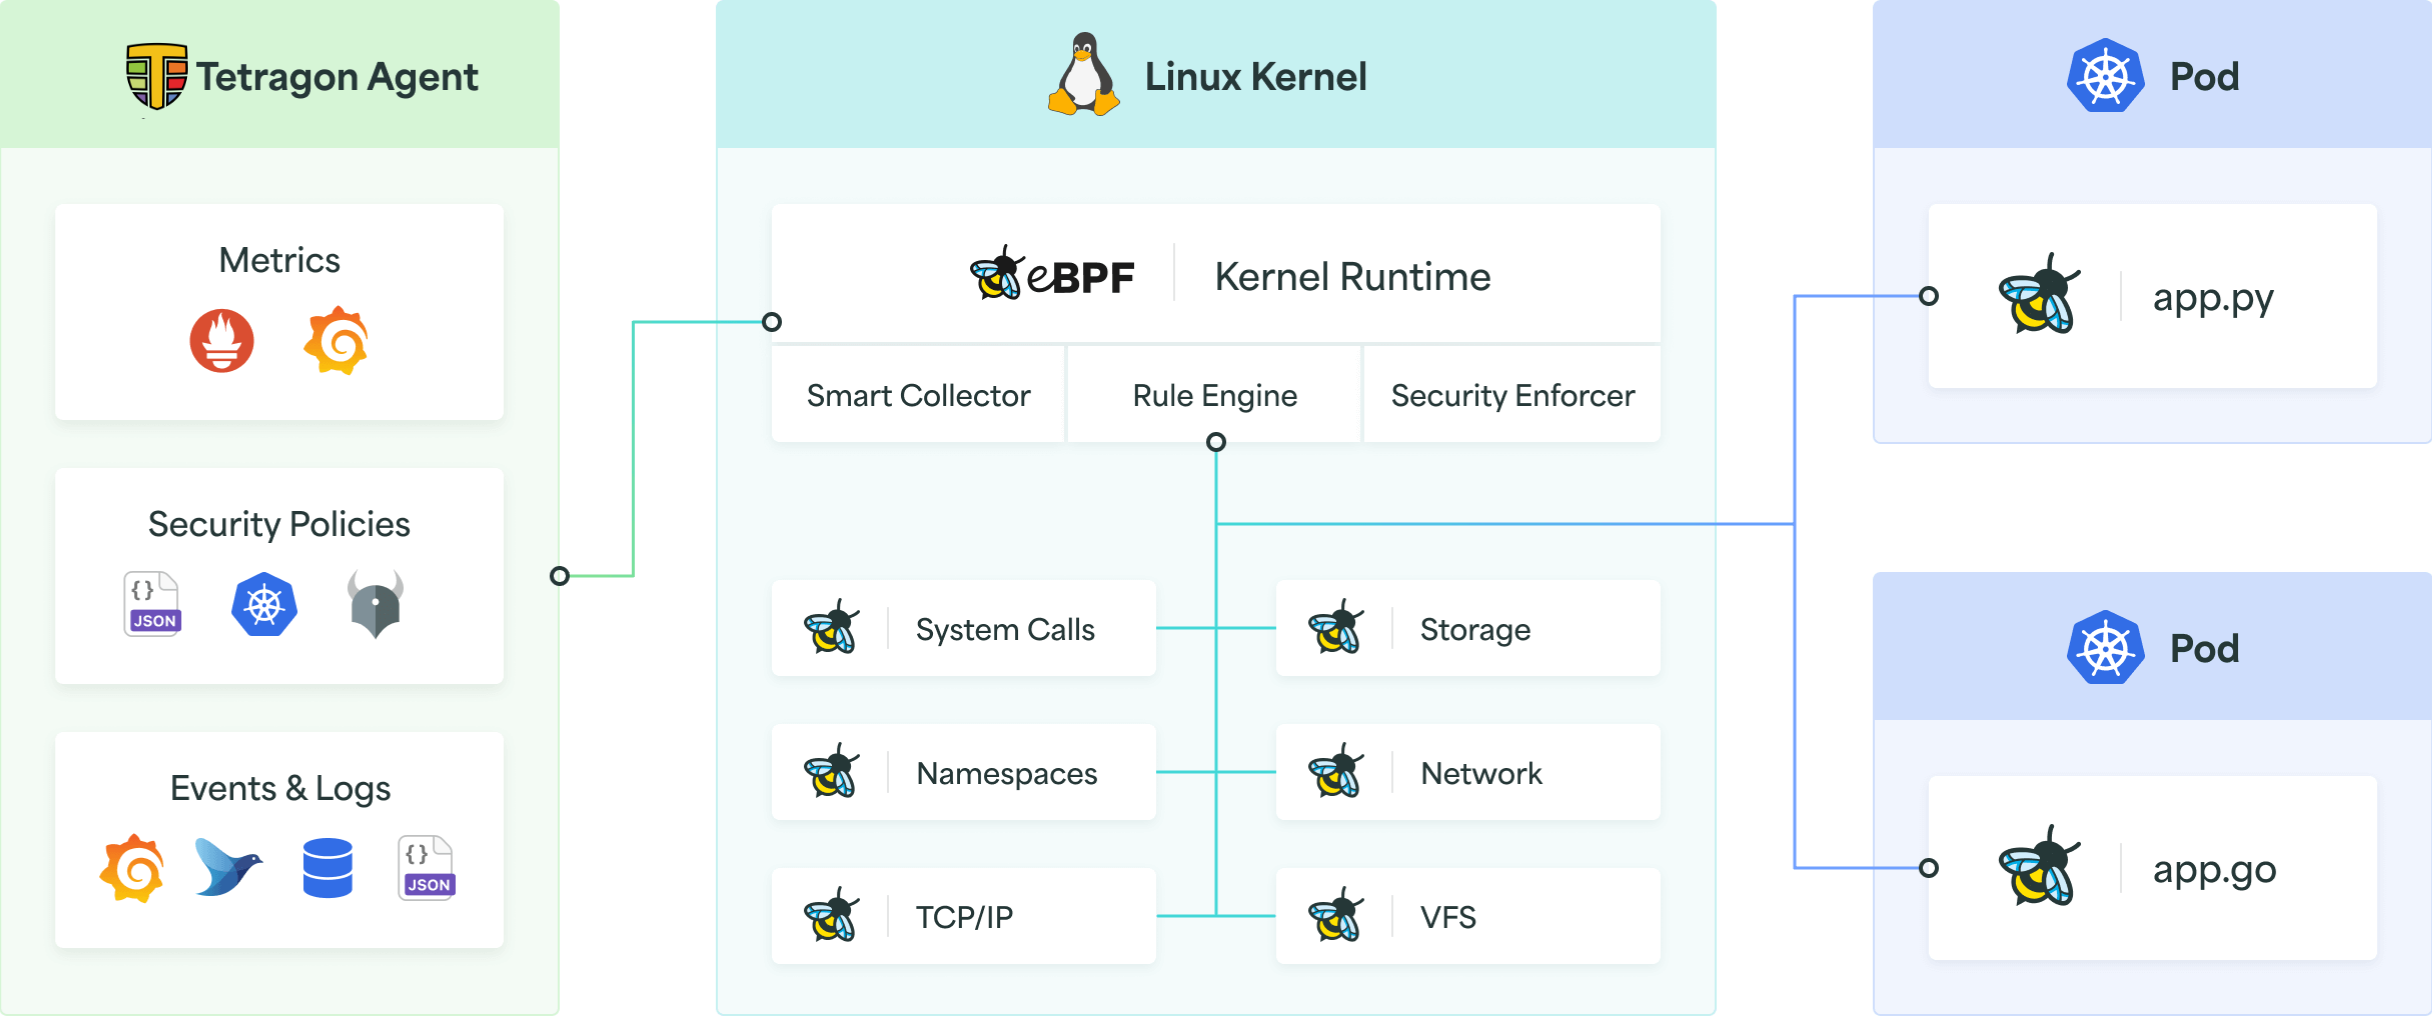
\includegraphics[scale=0.15]{images/tetragon.png}
\centering
\end{figure}

\end{frame}

\begin{frame}
\frametitle{\emph{Syscall} tooling}

Várias ferramentas fazem uso de \emph{syscalls} para monitorizar e responder a eventos relevantes de um ponto de vista de segurança. 

\pause
\begin{alertblock}{\textbf{TOCTOU}}
    Estas ferramentas são vulneráveis a ataques de \textbf{TOCTOU}, visto estarem normalmente na entrada da função chamada pelo \emph{kernel}.
\end{alertblock}


\end{frame}

\begin{frame}
\frametitle{BPF LSM}


\begin{figure}[x]
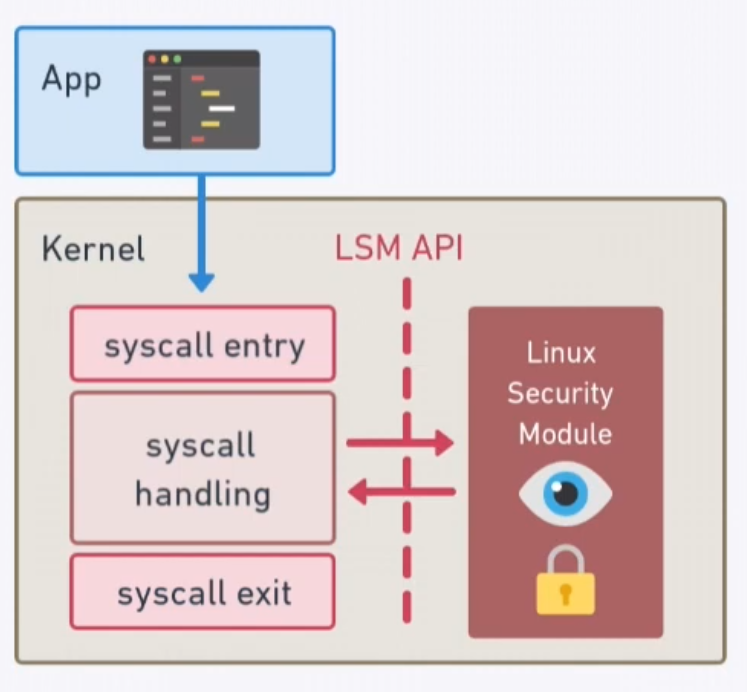
\includegraphics[scale=0.25]{images/lsm2.png}
\centering
\end{figure}

\end{frame}





\begin{frame}{}
  \centering \Huge
  \textbf{\emph{Demo}}
\end{frame}

\begin{frame}{}
  \centering \Huge
  \textbf{\emph{Trabalho futuro}}
\end{frame}

\begin{frame}{}
  \centering \Huge
  \textbf{\emph{Questões}}
\end{frame}



\end{document}
